\documentclass[a4paper,11pt]{article}
%@@@@@@@@@@@@@@@@@@@@@@@@@@@@@@@@@@@@@@@@@@@@@@@@@@@@@@@@@@@
%@@@@@@@@@@@@@@@@      PACOTES BÁSICOS		     @@@@@@@@@@
%@@@@@@@@@@@@@@@@@@@@@@@@@@@@@@@@@@@@@@@@@@@@@@@@@@@@@@@@@@@

\usepackage[T1]{fontenc}
\usepackage[utf8]{inputenc}
\usepackage{lmodern} 
\usepackage[portuguese]{babel}
\usepackage{amsmath}
\usepackage{array}
\usepackage{graphicx}				%para imagens
\usepackage{epstopdf} 				%resolve problemas eps-pdf
\usepackage{pict2e}				%%writting to images
%@@@@@@@@@@@@@@@@@@@@@@@@@@@@@@@@@@@@@@@@@@@@@@@@@@@@@@@@@@@
%@@@@@@@@@@@@@@@@     PACOTES NÃO TAOBÁSICOS		 @@@@@@@@@@
%@@@@@@@@@@@@@@@@@@@@@@@@@@@@@@@@@@@@@@@@@@@@@@@@@@@@@@@@@@@
\usepackage{fancyhdr}				% para o cabeçalho bonito
\usepackage{caption}					%para legendas
\usepackage{subcaption}				% e sublegendas
\usepackage{placeins} 				%controlar o lugar dos floats
\pagestyle{fancy} 					% número de pag e cabeçalho
\usepackage{txfonts} 				%fontes bonitas? acho que para o título
\usepackage[usenames]{color} 		% algo com gunplot e eps
\usepackage{ifthen}
\usepackage{xparse}
\graphicspath{{./../images/}{./../data/}{./graph/}}	% procura imagens nessa pasta
\usepackage{float} %%para definir ambiente gráfico
\newfloat{Gráfico}{hbtp}{lop}[section]
%\usepackage{undertilde}	%%para notação de vetor do yuri
\usepackage[import]{xy} % para escrever em imagens
\xyoption{import}

\usepackage{listings}
\lstset{frame=single,}
%@@@@@@@@@@@@@@@@@@@@@@@@@@@@@@@@@@@@@@@@@@@@@@@@@@@@@@@@@@@
%@@@@@@@@@@@@@@@@      Cabeçalho de cada página      @@@@@@@
%@@@@@@@@@@@@@@@@@@@@@@@@@@@@@@@@@@@@@@@@@@@@@@@@@@@@@@@@@@@
\setlength{\headheight}{25pt}%compila sem erro
	\fancyhead{}
	\fancyfoot{}
	\fancyhead[R]{Sistemas de Medição}%direito superior
	\fancyhead[L]{
\includegraphics[height=0.25in]{./../images/logo_unb.pdf}}%esquerda superior
	\fancyfoot[C]{\thepage}%baixo centro
%E: Even page, O: Odd page, L: Left field, C: Center field, R: Right field, H: Header, F: Footer
% em documentos com dois lados use LO, RO. como esse documento não tem lados essa opção é inútil


%@@@@@@@@@@@@@@@@@@@@@@@@@@@@@@@@@@@@@@@@@@@@@@@@@@@@@@@@@@@
%@@@@@@@@@@@@@@@@      NOVOS COMANDOS		      @@@@@@@@@
%@@@@@@@@@@@@@@@@@@@@@@@@@@@@@@@@@@@@@@@@@@@@@@@@@@@@@@@@@@@
\newcommand\undermat[2]
	{
	  \makebox[0pt][l]
	  	{$\smash{\underbrace{\phantom{%
    \begin{matrix}#2\end{matrix}}}_{\text{$#1$}}}$
    		}#2
    	}
    	
\newcommand{\HRule}
	{
	\rule{\linewidth}{0.5mm}
	}
	
\newcommand{\EmptyPage}
	{
	\thispagestyle{empty}
	\mbox{ }
	\newpage	
	} 
	
\newcommand{\MakeMyTitlePage}[4]
%%Argumentos: 
%1º Nome da Matéria
%2º subtítulo ex: experimento IV
%3º título
%4º autores
% exemplo de autores:
%	\begin{center} \large
%		\begin{tabular}{llr} \
%		& & \\[0.05cm]		
%		Professora & Nadia Maria de Liz Koche & \\
%		
%		Alunos:& & \\
%		& Juarez A.S.F 					& 11/0032829\\
%		& Sérgio Fernandes da Silva Reis & 11/0140257\\
%		& Jedhai Pimentel				& 09/0007883\\	[0.05cm]	
%		\end{tabular}
%	\end{center}
{
\begin{titlepage}
\begin{center}

% Upper part of the page. The '~' is needed because \\
% only works if a paragraph has started.

\includegraphics[width=\textwidth]{./../images/logo_unb.pdf}~\\[1cm]

\Huge #1\\[0.5cm]

\huge #2

% Title
\HRule \\[0.4cm]
{ \huge \bfseries  #3}\\[0.4cm]

\HRule \\[0.5cm]

{\large \today}


\vfill %%o que vier depois vai ao fim da páginda


%Autor e Professor
\begin{center} \large
#4
\end{center}

\end{center}
\end{titlepage}

\EmptyPage
\tableofcontents
\newpage

}
	
%@@@@@@@@@@@@@@@@@@@@@@@@@@@@@@@@@@@@@@@@@@@@@@@@@@@@@@@@@@@
%@@@@@@@@@@@@@@@@      NOVOS AMBIENTES		      @@@@@@@@@
%@@@@@@@@@@@@@@@@@@@@@@@@@@@@@@@@@@@@@@@@@@@@@@@@@@@@@@@@@@@
\newcounter{graph-c}
\setcounter{graph-c}{0}


%\NewDocumentEnvironment{Graph}{m}
 % {%antes
  %\addtocounter{graph-c}{1}
  %\begin{figure}
  %}
 %{
 %depois
%	\end{figure} 
%	\caption*{Grafico \arabic{graph-c} - #1}
 %}

















%inclui todosos pacotes utilizados

\newcommand{\MyBox}[1]
{
	\begin{tabular}{|l|}\hline
	  #1 \\ \hline	    
	\end{tabular} 	
}

\begin{document}



\MakeMyTitlePage
{Cálculo Numérico}
{Trabalho 2}
{Ajuste de Curvas, Derivação, Integração e Splines}
{%autores
		\begin{tabular}{llr} \
		& & \\[0.05cm]		
		Professor: & Yuri Dumaresq Sobral & \\
		
		Aluno:& & \\
		& Juarez A.S.F 					& 11/0032829\\

		\end{tabular}
}

\section*{Questão 1}

\paragraph{}Para o conjunto de dados da tabela 1 deseja-se
calcular os ajustes polinomiais de ordem 1,2,3,5 e 10.
 Ou seja, achar quais são os polinômios de ordem n $y_{n}(t)$ 
\begin{displaymath}
y_n(t) = \alpha_{0}n^{0} + \alpha_{1}n^{1} + \ldots 
									\alpha_{n}t^{n}
\end{displaymath}
que 
miniminizam o erro quadrático médio 
\begin{equation}
e_{n} = \sqrt{\sum _{i = 1}^{m} [y_{i} - y_{n}(t_{i})]^2}
\label{eq:erro}
\end{equation}

sobre o conjunto de m dados na forma $(t_{i}, y_{i})$. 
A tabela apresenta 17 desses pares, nesse caso m = 17. 
A função PolynomialFitting do anexo realiza o cálculo dos 
coeficientes e os resultados são plotados nos gráficos 
\ref{fig:quest1-a} e \ref{fig:quest1-b}. No primeiro gráfico
vemos os ajustes para n = 1,2 e 3. No segundo vemos n = 5 e 10.
Os resultados foram separados em dois gráficos para permitir 
melhor visualização das curvas. As tabelas de \ref{tab:quest1-X1} 
a \ref{tab:quest1-X10} mostram os coeficientes $\alpha_n$ calculados.

\paragraph{}Descrevemos brevemente o algoritmo utilizado.
Considere a expressão $[y_{i} - y_{n}(t_{i})]$. Pela fórmula
\ref{eq:erro} vemos que $e_n$ será mínimo quando essa expressão
for mínima, i.e.:$y_{i} = y_{n}(t_{i}), \forall 
t = \{ 1, 2, \ldots, m \}$, onde n é a ordem dada do polinômio  e m o número
de dados tomados. As incógnitas desse problema são os coeficientes $\alpha_j$,
com $j = {0, 1, \ldots, n}$. Esse sistema pode ser reescrito na forma $Ax = y$
com:

\begin{minipage}{0.3\textwidth}
\begin{displaymath}
	A_{\mbox{mx(n+1)}} = \left(
	\begin{array}{lllll}
	1 & t_1 & t_1^2 & \ldots & t_1^n \\
	1 & t_2 & t_2^2 & \ldots & t_2^n \\
	\vdots & \vdots & \vdots &\ddots  & \vdots \\
	1 & t_m & t_m^2 & \ldots & t_m^n \\
	\end{array}\right)
\end{displaymath}
\end{minipage}
\hspace{2 cm}
\begin{minipage}{0.3\textwidth}
\begin{displaymath}
	x_{\mbox{(n+1)x1}} = \left(
	\begin{array}{l}
	\alpha_0 \\
	\alpha_1 \\
	\vdots \\
	\alpha_n \\
	\end{array}\right)
\end{displaymath}
\end{minipage}
\begin{minipage}{0.3\textwidth}
\begin{displaymath}
	y_{\mbox{mx1}} = \left(
	\begin{array}{l}
	y_0 \\
	y_1 \\
	\vdots \\
	y_n \\
	\end{array}\right)
\end{displaymath}
\end{minipage}

\paragraph{}O sistema pode ser resolvido de diversas formas. Se quisermos
inverter matrizes podemos usar:

\begin{equation}
	x = (A^T A)^{-1}A^T y
	\label{eq:SolvingSystemGeral}
\end{equation}

\paragraph{} Podemos também usar as diversas técnicas de solução de sistemas
estudadas ao longo do curso. Para isso fazemos $D =A^T A$ e $E=(A^T y)$ e podemos
usar os métodos de Jacobi ou Gauss-Seidel por exemplo para resolver $Dx = E$

\paragraph{}Na equação \ref{eq:SolvingSystemGeral} a existência da inversa 
$(A^T A)^{-1}$ se baseia no fato de que a matriz A tem colunas linearmente
independentes, o que é garantido no caso em que existem ao menos 2 $t_i$'s 
diferentes entre si.

\paragraph{} No caso em que m = n+1 teremos a matriz A quadrada e o
erro dever ser zero. Isto é, o polinômio coincide perfeitamente com os dados
nos pontos tomados. Nesse caso temos o polinômio interpolador. Nos outros casos
a interpolação não é perfeita e temos apenas o polinômio de ordem n que melhor
se ajusta aos dados.

\paragraph{}Em nosso código o sistema é resolvido pela inversão de matrizes. 
A rotina foi implementada em C e o anexo contém todos os algoritmo usados,
inclusive os de interseção de matrizes,  multiplicação, soma e transposição.
Essas rotinas são consideradas auxiliares e portanto apresentadas separadamente
dos códigos principais para interpolação. 

\paragraph{}Os gráficos \ref{fig:quest1-a} e \ref{fig:quest1-b} nos mostram
 que a medida que aumenta a ordem n
do polinômio temos mais oscilações no fitting. Sem saber o que os dados
representam e para que serão usados é difícil decidir sobre qual o ajuste
mais adequado. Sem essa informação podemos apenas qualificar os ajustes quanto
aos erros quadráticos médios que deram origem ao método que
calculou as interpolações. A expressão \ref{eq:erro} pode ser 
calucalada para cada uma das curvas. Os resultados são apresentados na tabela
a seguir.

\begin{table}[!htp]
\centering
	\begin{tabular}{|l|l|}\hline
	n & $E_{n}$ \\ \hline
	 1	& 4.967 \\ \hline	
	 2	& 5.045\\ \hline	
	 3	& 5.861\\ \hline	
	 5	& 6.126\\ \hline	
	10	& 7.616\\ \hline	
	\end{tabular}
	\caption{Erro quadrático médio para n = 1,2,3,5 e 10}
	\label{tab:ERMS-quest1}
\end{table}

\paragraph{}Vemos que nesse caso aumentar o grau do polinômio de
interpolação nos deu um maior erro quadrático médio. Baseado nesses
dados podemos dizer que o melhor ajuste dentre esses 5 feitos é o 
de primeira ordem. 

\FloatBarrier
\begin{figure}[!htp]
	\begin{subfigure}[!htp]{0.5\textwidth}
	% GNUPLOT: LaTeX picture with Postscript
\begingroup
  \fontfamily{phv}%
  \selectfont
\definecolor{t}{rgb}{0.5,0.5,0.5}
  \makeatletter
  \providecommand\color[2][]{%
    \GenericError{(gnuplot) \space\space\space\@spaces}{%
      Package color not loaded in conjunction with
      terminal option `colourtext'%
    }{See the gnuplot documentation for explanation.%
    }{Either use 'blacktext' in gnuplot or load the package
      color.sty in LaTeX.}%
    \renewcommand\color[2][]{}%
  }%
  \providecommand\includegraphics[2][]{%
    \GenericError{(gnuplot) \space\space\space\@spaces}{%
      Package graphicx or graphics not loaded%
    }{See the gnuplot documentation for explanation.%
    }{The gnuplot epslatex terminal needs graphicx.sty or graphics.sty.}%
    \renewcommand\includegraphics[2][]{}%
  }%
  \providecommand\rotatebox[2]{#2}%
  \@ifundefined{ifGPcolor}{%
    \newif\ifGPcolor
    \GPcolortrue
  }{}%
  \@ifundefined{ifGPblacktext}{%
    \newif\ifGPblacktext
    \GPblacktextfalse
  }{}%
  % define a \g@addto@macro without @ in the name:
  \let\gplgaddtomacro\g@addto@macro
  % define empty templates for all commands taking text:
  \gdef\gplbacktext{}%
  \gdef\gplfronttext{}%
  \makeatother
  \ifGPblacktext
    % no textcolor at all
    \def\colorrgb#1{}%
    \def\colorgray#1{}%
  \else
    % gray or color?
    \ifGPcolor
      \def\colorrgb#1{\color[rgb]{#1}}%
      \def\colorgray#1{\color[gray]{#1}}%
      \expandafter\def\csname LTw\endcsname{\color{white}}%
      \expandafter\def\csname LTb\endcsname{\color{black}}%
      \expandafter\def\csname LTa\endcsname{\color{black}}%
      \expandafter\def\csname LT0\endcsname{\color[rgb]{1,0,0}}%
      \expandafter\def\csname LT1\endcsname{\color[rgb]{0,1,0}}%
      \expandafter\def\csname LT2\endcsname{\color[rgb]{0,0,1}}%
      \expandafter\def\csname LT3\endcsname{\color[rgb]{1,0,1}}%
      \expandafter\def\csname LT4\endcsname{\color[rgb]{0,1,1}}%
      \expandafter\def\csname LT5\endcsname{\color[rgb]{1,1,0}}%
      \expandafter\def\csname LT6\endcsname{\color[rgb]{0,0,0}}%
      \expandafter\def\csname LT7\endcsname{\color[rgb]{1,0.3,0}}%
      \expandafter\def\csname LT8\endcsname{\color[rgb]{0.5,0.5,0.5}}%
    \else
      % gray
      \def\colorrgb#1{\color{black}}%
      \def\colorgray#1{\color[gray]{#1}}%
      \expandafter\def\csname LTw\endcsname{\color{white}}%
      \expandafter\def\csname LTb\endcsname{\color{black}}%
      \expandafter\def\csname LTa\endcsname{\color{black}}%
      \expandafter\def\csname LT0\endcsname{\color{black}}%
      \expandafter\def\csname LT1\endcsname{\color{black}}%
      \expandafter\def\csname LT2\endcsname{\color{black}}%
      \expandafter\def\csname LT3\endcsname{\color{black}}%
      \expandafter\def\csname LT4\endcsname{\color{black}}%
      \expandafter\def\csname LT5\endcsname{\color{black}}%
      \expandafter\def\csname LT6\endcsname{\color{black}}%
      \expandafter\def\csname LT7\endcsname{\color{black}}%
      \expandafter\def\csname LT8\endcsname{\color{black}}%
    \fi
  \fi
  \setlength{\unitlength}{0.0500bp}%
  \begin{picture}(7936.00,5668.00)%
    \gplgaddtomacro\gplbacktext{%
      \csname LTb\endcsname%
      \put(558,1476){\makebox(0,0)[r]{\strut{} 0}}%
      \put(558,1882){\makebox(0,0)[r]{\strut{} 1}}%
      \put(558,2287){\makebox(0,0)[r]{\strut{} 2}}%
      \put(558,2693){\makebox(0,0)[r]{\strut{} 3}}%
      \put(558,3099){\makebox(0,0)[r]{\strut{} 4}}%
      \put(558,3504){\makebox(0,0)[r]{\strut{} 5}}%
      \put(558,3910){\makebox(0,0)[r]{\strut{} 6}}%
      \put(558,4316){\makebox(0,0)[r]{\strut{} 7}}%
      \put(558,4721){\makebox(0,0)[r]{\strut{} 8}}%
      \put(558,5127){\makebox(0,0)[r]{\strut{} 9}}%
      \put(666,1296){\makebox(0,0){\strut{} 0}}%
      \put(1438,1296){\makebox(0,0){\strut{} 0.2}}%
      \put(2209,1296){\makebox(0,0){\strut{} 0.4}}%
      \put(2981,1296){\makebox(0,0){\strut{} 0.6}}%
      \put(3753,1296){\makebox(0,0){\strut{} 0.8}}%
      \put(4524,1296){\makebox(0,0){\strut{} 1}}%
      \put(5296,1296){\makebox(0,0){\strut{} 1.2}}%
      \put(6068,1296){\makebox(0,0){\strut{} 1.4}}%
      \put(6839,1296){\makebox(0,0){\strut{} 1.6}}%
      \put(7611,1296){\makebox(0,0){\strut{} 1.8}}%
      \put(144,3301){\makebox(0,0){\strut{}y(t)}}%
      \put(4138,1026){\makebox(0,0){\strut{}t}}%
      \put(4138,5397){\makebox(0,0){\strut{}Ajuste Polinomial}}%
    }%
    \gplgaddtomacro\gplfronttext{%
      \csname LTb\endcsname%
      \put(4377,693){\makebox(0,0)[r]{\strut{}$y_{1}(t)$}}%
      \csname LTb\endcsname%
      \put(4377,513){\makebox(0,0)[r]{\strut{}$y_{2}(t)$}}%
      \csname LTb\endcsname%
      \put(4377,333){\makebox(0,0)[r]{\strut{}$y_{3}(t)$}}%
      \csname LTb\endcsname%
      \put(4377,153){\makebox(0,0)[r]{\strut{}data points}}%
    }%
    \gplbacktext
    \put(0,0){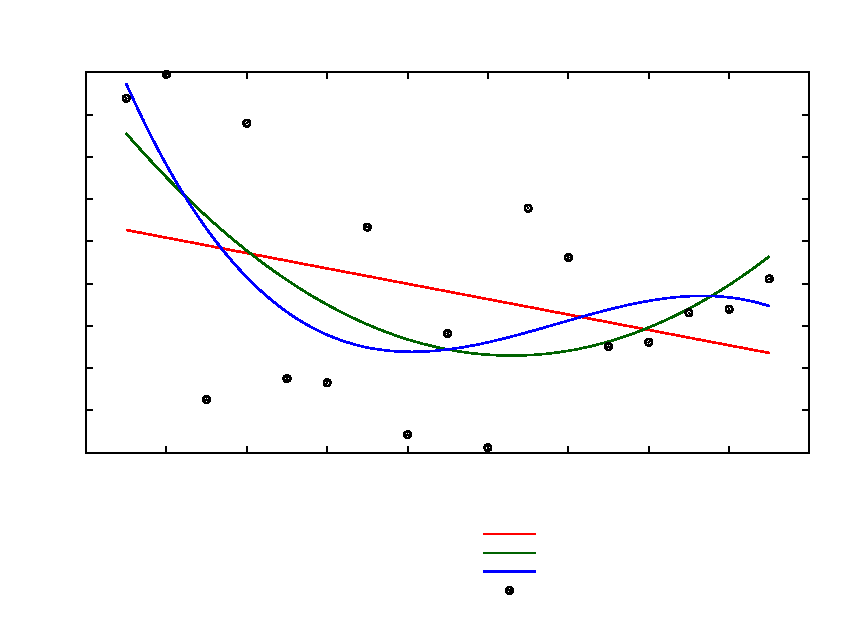
\includegraphics{./../LaTeX/graph/quest1-a}}%
    \gplfronttext
  \end{picture}%
\endgroup

	\caption{Fitting para n = 1,2 e 3}
	\label{fig:quest1-a}
	\end{subfigure}

	\begin{subfigure}[!htp]{0.5\textwidth}
	% GNUPLOT: LaTeX picture with Postscript
\begingroup
  \fontfamily{phv}%
  \selectfont
\definecolor{t}{rgb}{0.5,0.5,0.5}
  \makeatletter
  \providecommand\color[2][]{%
    \GenericError{(gnuplot) \space\space\space\@spaces}{%
      Package color not loaded in conjunction with
      terminal option `colourtext'%
    }{See the gnuplot documentation for explanation.%
    }{Either use 'blacktext' in gnuplot or load the package
      color.sty in LaTeX.}%
    \renewcommand\color[2][]{}%
  }%
  \providecommand\includegraphics[2][]{%
    \GenericError{(gnuplot) \space\space\space\@spaces}{%
      Package graphicx or graphics not loaded%
    }{See the gnuplot documentation for explanation.%
    }{The gnuplot epslatex terminal needs graphicx.sty or graphics.sty.}%
    \renewcommand\includegraphics[2][]{}%
  }%
  \providecommand\rotatebox[2]{#2}%
  \@ifundefined{ifGPcolor}{%
    \newif\ifGPcolor
    \GPcolortrue
  }{}%
  \@ifundefined{ifGPblacktext}{%
    \newif\ifGPblacktext
    \GPblacktextfalse
  }{}%
  % define a \g@addto@macro without @ in the name:
  \let\gplgaddtomacro\g@addto@macro
  % define empty templates for all commands taking text:
  \gdef\gplbacktext{}%
  \gdef\gplfronttext{}%
  \makeatother
  \ifGPblacktext
    % no textcolor at all
    \def\colorrgb#1{}%
    \def\colorgray#1{}%
  \else
    % gray or color?
    \ifGPcolor
      \def\colorrgb#1{\color[rgb]{#1}}%
      \def\colorgray#1{\color[gray]{#1}}%
      \expandafter\def\csname LTw\endcsname{\color{white}}%
      \expandafter\def\csname LTb\endcsname{\color{black}}%
      \expandafter\def\csname LTa\endcsname{\color{black}}%
      \expandafter\def\csname LT0\endcsname{\color[rgb]{1,0,0}}%
      \expandafter\def\csname LT1\endcsname{\color[rgb]{0,1,0}}%
      \expandafter\def\csname LT2\endcsname{\color[rgb]{0,0,1}}%
      \expandafter\def\csname LT3\endcsname{\color[rgb]{1,0,1}}%
      \expandafter\def\csname LT4\endcsname{\color[rgb]{0,1,1}}%
      \expandafter\def\csname LT5\endcsname{\color[rgb]{1,1,0}}%
      \expandafter\def\csname LT6\endcsname{\color[rgb]{0,0,0}}%
      \expandafter\def\csname LT7\endcsname{\color[rgb]{1,0.3,0}}%
      \expandafter\def\csname LT8\endcsname{\color[rgb]{0.5,0.5,0.5}}%
    \else
      % gray
      \def\colorrgb#1{\color{black}}%
      \def\colorgray#1{\color[gray]{#1}}%
      \expandafter\def\csname LTw\endcsname{\color{white}}%
      \expandafter\def\csname LTb\endcsname{\color{black}}%
      \expandafter\def\csname LTa\endcsname{\color{black}}%
      \expandafter\def\csname LT0\endcsname{\color{black}}%
      \expandafter\def\csname LT1\endcsname{\color{black}}%
      \expandafter\def\csname LT2\endcsname{\color{black}}%
      \expandafter\def\csname LT3\endcsname{\color{black}}%
      \expandafter\def\csname LT4\endcsname{\color{black}}%
      \expandafter\def\csname LT5\endcsname{\color{black}}%
      \expandafter\def\csname LT6\endcsname{\color{black}}%
      \expandafter\def\csname LT7\endcsname{\color{black}}%
      \expandafter\def\csname LT8\endcsname{\color{black}}%
    \fi
  \fi
  \setlength{\unitlength}{0.0500bp}%
  \begin{picture}(7936.00,5668.00)%
    \gplgaddtomacro\gplbacktext{%
      \csname LTb\endcsname%
      \put(666,1296){\makebox(0,0)[r]{\strut{} 0}}%
      \put(666,1935){\makebox(0,0)[r]{\strut{} 2}}%
      \put(666,2573){\makebox(0,0)[r]{\strut{} 4}}%
      \put(666,3212){\makebox(0,0)[r]{\strut{} 6}}%
      \put(666,3850){\makebox(0,0)[r]{\strut{} 8}}%
      \put(666,4489){\makebox(0,0)[r]{\strut{} 10}}%
      \put(666,5127){\makebox(0,0)[r]{\strut{} 12}}%
      \put(774,1116){\makebox(0,0){\strut{} 0}}%
      \put(1534,1116){\makebox(0,0){\strut{} 0.2}}%
      \put(2293,1116){\makebox(0,0){\strut{} 0.4}}%
      \put(3053,1116){\makebox(0,0){\strut{} 0.6}}%
      \put(3813,1116){\makebox(0,0){\strut{} 0.8}}%
      \put(4572,1116){\makebox(0,0){\strut{} 1}}%
      \put(5332,1116){\makebox(0,0){\strut{} 1.2}}%
      \put(6092,1116){\makebox(0,0){\strut{} 1.4}}%
      \put(6851,1116){\makebox(0,0){\strut{} 1.6}}%
      \put(7611,1116){\makebox(0,0){\strut{} 1.8}}%
      \put(144,3211){\makebox(0,0){\strut{}y(t)}}%
      \put(4192,846){\makebox(0,0){\strut{}t}}%
      \put(4192,5397){\makebox(0,0){\strut{}Ajuste Polinomial}}%
    }%
    \gplgaddtomacro\gplfronttext{%
      \csname LTb\endcsname%
      \put(4431,513){\makebox(0,0)[r]{\strut{}$y_{5}(t)$}}%
      \csname LTb\endcsname%
      \put(4431,333){\makebox(0,0)[r]{\strut{}$y_{10}(t)$}}%
      \csname LTb\endcsname%
      \put(4431,153){\makebox(0,0)[r]{\strut{}data points}}%
    }%
    \gplbacktext
    \put(0,0){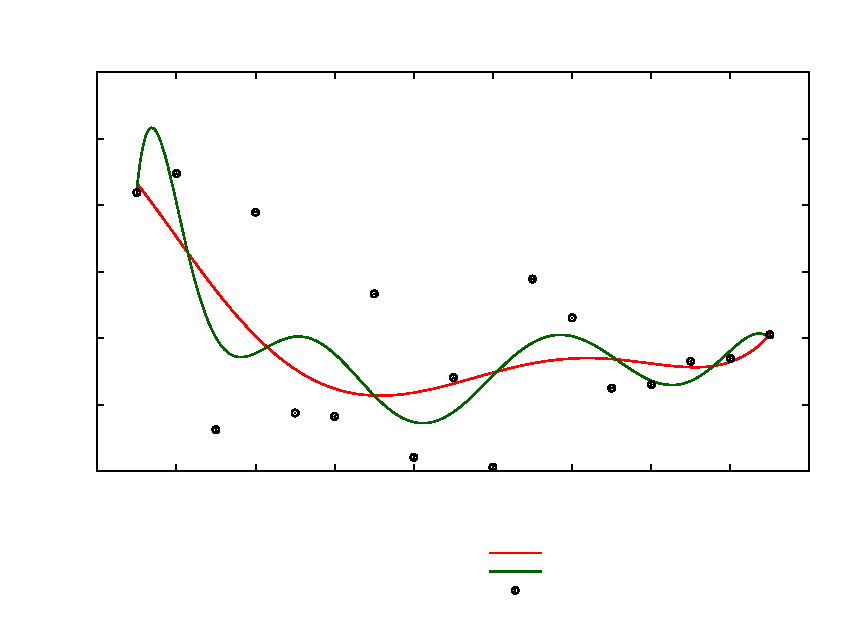
\includegraphics{./../LaTeX/graph/quest1-b}}%
    \gplfronttext
  \end{picture}%
\endgroup

	\caption{Fitting para n = 5, 10}
	\label{fig:quest1-b}	
	\end{subfigure}
	\caption{Gráficos da questão 1}
\end{figure}
\FloatBarrier

\FloatBarrier
\begin{table}
\parbox{.45\linewidth}
		{
		\centering
		\begin{tabular}{|l|l|}\hline
			n & $\alpha_{n}$ \\ \hline
					 0 &  5.449156 \\ \hline 
		 1 &  -1.819039 \\ \hline 
		 1 &  -1.819039 \\ \hline 

		\end{tabular}
		\caption{coeficientes de $y_1(t)$}
		\label{tab:quest1-X1}
		}
\parbox{.45\linewidth}
	{
	\centering
		\begin{tabular}{|l|l|}\hline
			n & $\alpha_{n}$ \\ \hline
					 0 &  8.706067 \\ \hline 
		 1 &  -12.104022 \\ \hline 
		 2 &  5.713879 \\ \hline 
		 2 &  5.713879 \\ \hline 

		\end{tabular}
		\caption{coeficientes de $y_2(t)$}
		\label{tab:quest1-X2}	
	}

\parbox{.45\linewidth}
	{
	\centering
		\begin{tabular}{|l|l|}\hline
			n & $\alpha_{n}$ \\ \hline
					 0 &  11.099895 \\ \hline 
		 1 &  -26.103014 \\ \hline 
		 2 &  24.612518 \\ \hline 
		 3 &  -6.999496 \\ \hline 
		 3 &  -6.999496 \\ \hline 

		\end{tabular}
		\caption{coeficientes de $y_3(t)$}
		\label{tab:quest1-X3}
	}
\parbox{.45\linewidth}
	{
	\centering
		\begin{tabular}{|l|l|}\hline
			n & $\alpha_{n}$ \\ \hline
					 0 &  9.882275 \\ \hline 
		 1 &  -8.734146 \\ \hline 
		 2 &  -44.816147 \\ \hline 
		 3 &  102.115150 \\ \hline 
		 4 &  -72.629829 \\ \hline 
		 5 &  17.150402 \\ \hline 
		 5 &  17.150402 \\ \hline 

		\end{tabular}
		\caption{coeficientes de $y_5(t)$}
		\label{tab:quest1-X5}
	}
	
\parbox{.45\linewidth}
	{
	\centering
		\begin{tabular}{|l|l|}\hline
			n & $\alpha_{n}$ \\ \hline
					 0 &  -41.381470 \\ \hline 
		 1 &  1116.054321 \\ \hline 
		 2 &  -9137.643555 \\ \hline 
		 3 &  37257.980469 \\ \hline 
		 4 &  -87894.031250 \\ \hline 
		 5 &  128680.648438 \\ \hline 
		 6 &  -120650.898438 \\ \hline 
		 7 &  72604.195312 \\ \hline 
		 8 &  -27166.693359 \\ \hline 
		 9 &  5766.708008 \\ \hline 
		 10 &  -532.068542 \\ \hline 
		 10 &  -532.068542 \\ \hline 

		\end{tabular}
		\caption{coeficientes de $y_{10}(t)$}
		\label{tab:quest1-X10}
	}

\end{table}
\FloatBarrier


% GNUPLOT: LaTeX picture with Postscript
\begingroup
  \fontfamily{phv}%
  \selectfont
\definecolor{t}{rgb}{0.5,0.5,0.5}
  \makeatletter
  \providecommand\color[2][]{%
    \GenericError{(gnuplot) \space\space\space\@spaces}{%
      Package color not loaded in conjunction with
      terminal option `colourtext'%
    }{See the gnuplot documentation for explanation.%
    }{Either use 'blacktext' in gnuplot or load the package
      color.sty in LaTeX.}%
    \renewcommand\color[2][]{}%
  }%
  \providecommand\includegraphics[2][]{%
    \GenericError{(gnuplot) \space\space\space\@spaces}{%
      Package graphicx or graphics not loaded%
    }{See the gnuplot documentation for explanation.%
    }{The gnuplot epslatex terminal needs graphicx.sty or graphics.sty.}%
    \renewcommand\includegraphics[2][]{}%
  }%
  \providecommand\rotatebox[2]{#2}%
  \@ifundefined{ifGPcolor}{%
    \newif\ifGPcolor
    \GPcolortrue
  }{}%
  \@ifundefined{ifGPblacktext}{%
    \newif\ifGPblacktext
    \GPblacktextfalse
  }{}%
  % define a \g@addto@macro without @ in the name:
  \let\gplgaddtomacro\g@addto@macro
  % define empty templates for all commands taking text:
  \gdef\gplbacktext{}%
  \gdef\gplfronttext{}%
  \makeatother
  \ifGPblacktext
    % no textcolor at all
    \def\colorrgb#1{}%
    \def\colorgray#1{}%
  \else
    % gray or color?
    \ifGPcolor
      \def\colorrgb#1{\color[rgb]{#1}}%
      \def\colorgray#1{\color[gray]{#1}}%
      \expandafter\def\csname LTw\endcsname{\color{white}}%
      \expandafter\def\csname LTb\endcsname{\color{black}}%
      \expandafter\def\csname LTa\endcsname{\color{black}}%
      \expandafter\def\csname LT0\endcsname{\color[rgb]{1,0,0}}%
      \expandafter\def\csname LT1\endcsname{\color[rgb]{0,1,0}}%
      \expandafter\def\csname LT2\endcsname{\color[rgb]{0,0,1}}%
      \expandafter\def\csname LT3\endcsname{\color[rgb]{1,0,1}}%
      \expandafter\def\csname LT4\endcsname{\color[rgb]{0,1,1}}%
      \expandafter\def\csname LT5\endcsname{\color[rgb]{1,1,0}}%
      \expandafter\def\csname LT6\endcsname{\color[rgb]{0,0,0}}%
      \expandafter\def\csname LT7\endcsname{\color[rgb]{1,0.3,0}}%
      \expandafter\def\csname LT8\endcsname{\color[rgb]{0.5,0.5,0.5}}%
    \else
      % gray
      \def\colorrgb#1{\color{black}}%
      \def\colorgray#1{\color[gray]{#1}}%
      \expandafter\def\csname LTw\endcsname{\color{white}}%
      \expandafter\def\csname LTb\endcsname{\color{black}}%
      \expandafter\def\csname LTa\endcsname{\color{black}}%
      \expandafter\def\csname LT0\endcsname{\color{black}}%
      \expandafter\def\csname LT1\endcsname{\color{black}}%
      \expandafter\def\csname LT2\endcsname{\color{black}}%
      \expandafter\def\csname LT3\endcsname{\color{black}}%
      \expandafter\def\csname LT4\endcsname{\color{black}}%
      \expandafter\def\csname LT5\endcsname{\color{black}}%
      \expandafter\def\csname LT6\endcsname{\color{black}}%
      \expandafter\def\csname LT7\endcsname{\color{black}}%
      \expandafter\def\csname LT8\endcsname{\color{black}}%
    \fi
  \fi
  \setlength{\unitlength}{0.0500bp}%
  \begin{picture}(7936.00,5668.00)%
    \gplgaddtomacro\gplbacktext{%
      \csname LTb\endcsname%
      \put(882,1116){\makebox(0,0)[r]{\strut{}-1400}}%
      \put(882,1617){\makebox(0,0)[r]{\strut{}-1200}}%
      \put(882,2119){\makebox(0,0)[r]{\strut{}-1000}}%
      \put(882,2620){\makebox(0,0)[r]{\strut{}-800}}%
      \put(882,3121){\makebox(0,0)[r]{\strut{}-600}}%
      \put(882,3623){\makebox(0,0)[r]{\strut{}-400}}%
      \put(882,4124){\makebox(0,0)[r]{\strut{}-200}}%
      \put(882,4626){\makebox(0,0)[r]{\strut{} 0}}%
      \put(882,5127){\makebox(0,0)[r]{\strut{} 200}}%
      \put(990,936){\makebox(0,0){\strut{} 0}}%
      \put(1726,936){\makebox(0,0){\strut{} 0.2}}%
      \put(2461,936){\makebox(0,0){\strut{} 0.4}}%
      \put(3197,936){\makebox(0,0){\strut{} 0.6}}%
      \put(3933,936){\makebox(0,0){\strut{} 0.8}}%
      \put(4668,936){\makebox(0,0){\strut{} 1}}%
      \put(5404,936){\makebox(0,0){\strut{} 1.2}}%
      \put(6140,936){\makebox(0,0){\strut{} 1.4}}%
      \put(6875,936){\makebox(0,0){\strut{} 1.6}}%
      \put(7611,936){\makebox(0,0){\strut{} 1.8}}%
      \put(144,3121){\makebox(0,0){\strut{}y(t)}}%
      \put(4300,666){\makebox(0,0){\strut{}t}}%
      \put(4300,5397){\makebox(0,0){\strut{}Ajuste Polinomial}}%
    }%
    \gplgaddtomacro\gplfronttext{%
      \csname LTb\endcsname%
      \put(4539,333){\makebox(0,0)[r]{\strut{}$y_{16}(t)$}}%
      \csname LTb\endcsname%
      \put(4539,153){\makebox(0,0)[r]{\strut{}data points}}%
    }%
    \gplbacktext
    \put(0,0){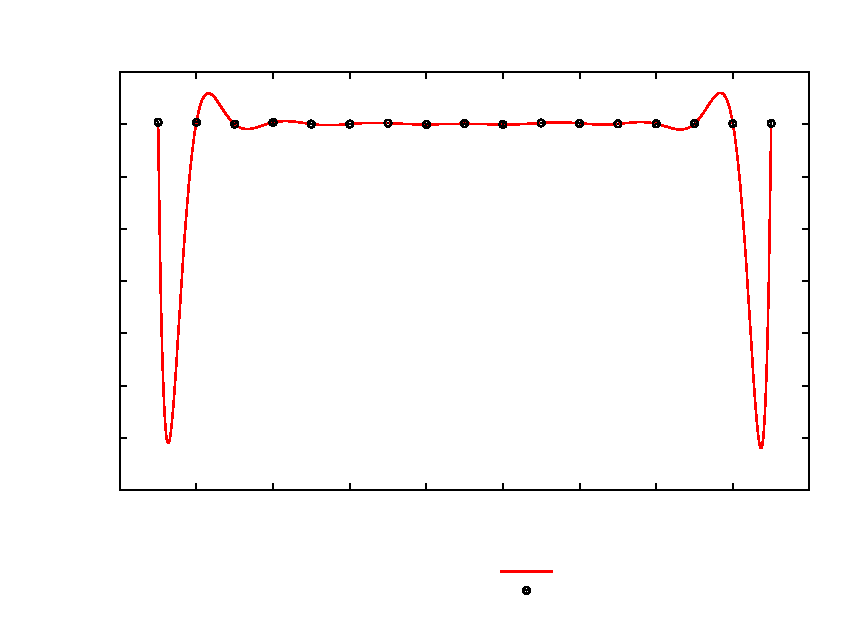
\includegraphics{./../LaTeX/graph/quest2}}%
    \gplfronttext
  \end{picture}%
\endgroup

\section*{Questão 3}

\paragraph{}Primeiro vamos derivar as equações de diferenças finitas de segunda ordem 
para a primeira e a segunda derivada. Para isso escrevamos a fórmula de Taylor de primeira 
, segunda e terceira ordem:

\begin{equation}
  \begin{array}{l}
      f(x_0 + h) = \frac{f^{(0)}(x_0)h^0}{0!} + 
          \frac{f^{(2)}(x_0)h^2}{2!} + \frac{f^{(2)}(\xi )h^2}{2!} \\
      f(x_0 + h) = \frac{f^{(0)}(x_0)h^0}{0!} + 
          \frac{f^{(2)}(x_0)h^2}{2!} + \frac{f^{(2)}(x_0)h^2}{2!} 
              + \frac{f^{(3)}(\xi)h^3}{3!}\\
      f(x_0 + h) = \frac{f^{(0)}(x_0)h^0}{0!} + 
          \frac{f^{(2)}(x_0)h^2}{2!} + \frac{f^{(2)}(x_0)h^2}{2!} 
              + \frac{f^{(3)}(x_0)h^3}{3!}
              +  \frac{f^{(4)}(\xi)h^4}{4!}\\

  \end{array}
\end{equation}

onde $\xi \in (x_0, h)$ nos dois casos. Vamos rescrever essas equações com a notação O(h):

\begin{equation}
  \begin{array}{l}
      f(x_0 + h) = \frac{f^{(0)}(x_0)h^0}{0!} + 
          \frac{f^{(2)}(x_0)h^2}{2!} + O(h^2) \\
      f(x_0 + h) = \frac{f^{(0)}(x_0)h^0}{0!} + 
          \frac{f^{(2)}(x_0)h^2}{2!} + \frac{f^{(2)}(x_0)h^2}{2!} 
              + O(h^3)\\
      f(x_0 + h) = \frac{f^{(0)}(x_0)h^0}{0!} + 
          \frac{f^{(2)}(x_0)h^2}{2!} + \frac{f^{(2)}(x_0)h^2}{2!} 
              + \frac{f^{(3)}(x_0)h^3}{3!}
               + O(h^4)\\
  \end{array}
\end{equation}

Usando a expressão com $O(h^4)$ e avaliando em f(x-h) e f(x+4) temos:
\begin{equation}
  f(x+h) + f(x-h) = 2f(x) + f^{(2)}h^2 + O(h^4)
\end{equation}

de onde obtemos:
\begin{equation}
  f^{(2)}(x) = \frac{f(x+h) - 2f(x) + f(x-h)}{h^2} + O(h^2)
\end{equation}

Essa é a expressão de diferenças finitas para a segunda derivada nos pontos interiores.
Fazendo $h =\triangle t$ esse método é $O(\triangle t^2)$. O mesmo procedimento
refeito com a expressão de Taylor com $O(h ^3)$ nos dá:

\begin{equation}
  f^{(1)}(x) = \frac{f(x+h) - f(x-h)}{2h} + O(h^2)
\end{equation}

Essa será a fórmula usada para a primeira derivada nos pontos interiores. Para os
pontos de fronteira teremos problemas, uma vez que $x_0-h$ e $x_n+h$ não estão tabelados
e seriam necessários para as fórmulas até aqui descritas. Procedimentos semelhantes
analisando mais pontos nos dão as seguinte fórmulas de diferenças finitas de
segunda ordem para frente:

\begin{equation}
  \begin{array}{l}
  f^{(1)}(x) = \frac{-\frac{3}{2}f(x) + 2f(x+h) -\frac{1}{2} f(x+2h}{h} + O(h^2) \\
  f^{(2)}(x) = \frac{2f(x) -5 f(x+h) +4 f(x+2h) - f(x+3h}{h} + O(h^2) \\
  \end{array}
\end{equation}

e as diferenças finitas de segunda ordem para trás:
\begin{equation}
  \begin{array}{l}
  f^{(1)}(x) = \frac{\frac{3}{2}f(x) - 2f(x-h) +\frac{1}{2} f(x-2h}{h} + O(h^2) \\
  f^{(2)}(x) = \frac{2f(x) -5 f(x-h) +4 f(x-2h) - f(x-3h}{h} + O(h^2) \\
  \end{array}
\end{equation}

Essa fórmulas serão usadas para o cálculo das derivadas primeiras e segundas nas extremidades.
O código é implementado em C e o resultado mostrado a seguir.

\FloatBarrier
\begin{table}
\parbox{.45\linewidth}
		{
		\centering
		\begin{tabular}{|l|l|}\hline
			t & $f^{(1)}(t)$ \\ \hline
					 0.1 &  47.062092 \\ \hline 
		 0.2 &  -35.654472 \\ \hline 
		 0.3 &  -5.798364 \\ \hline 
		 0.4 &  2.509927 \\ \hline 
		 0.5 &  -30.692114 \\ \hline 
		 0.6 &  17.910242 \\ \hline 
		 0.7 &  -6.173170 \\ \hline 
		 0.8 &  -12.601877 \\ \hline 
		 0.9 &  -1.512384 \\ \hline 
		 1.0 &  14.839912 \\ \hline 
		 1.1 &  22.500589 \\ \hline 
		 1.2 &  -16.399300 \\ \hline 
		 1.3 &  -10.041074 \\ \hline 
		 1.4 &  4.017377 \\ \hline 
		 1.5 &  3.913653 \\ \hline 
		 1.6 &  4.011237 \\ \hline 
		 1.7 &  10.324777 \\ \hline 
		 1.7 &  10.324777 \\ \hline 

		\end{tabular}
		\caption{Primeira derivada}
		\label{tab:quest1-X1}
		}
\parbox{.45\linewidth}
	{
	\centering
		\begin{tabular}{|l|l|}\hline
			t & $f^{(2)}(t)$ \\ \hline
					 0.1 &  -3078.619141 \\ \hline 
		 0.2 &  -827.165649 \\ \hline 
		 0.3 &  1424.287842 \\ \hline 
		 0.4 &  -1258.121948 \\ \hline 
		 0.5 &  594.081177 \\ \hline 
		 0.6 &  377.965942 \\ \hline 
		 0.7 &  -859.634155 \\ \hline 
		 0.8 &  731.060059 \\ \hline 
		 0.9 &  -509.270203 \\ \hline 
		 1.0 &  836.316101 \\ \hline 
		 1.1 &  -683.102539 \\ \hline 
		 1.2 &  -94.895279 \\ \hline 
		 1.3 &  222.059799 \\ \hline 
		 1.4 &  59.109219 \\ \hline 
		 1.5 &  -61.183701 \\ \hline 
		 1.6 &  63.135391 \\ \hline 
		 1.7 &  187.454483 \\ \hline 
		 1.7 &  187.454483 \\ \hline 

		\end{tabular}
		\caption{Segunda derivada}
		\label{tab:quest1-X2}	
	}
	

\end{table}

\FloatBarrier

\paragraph{}O ajuste escolhido como o melhor na questão 2 tem primeira derivada constante e igual a
$\alpha_1 = -1.819038$ e segunda derivada constante igual a 0. Quanto a derivada
primeira podemos dizer apenas que os valores tem mesma ordem de grandeza. Já a segunda
derivada difere totalmente. As duas aproximações levaram a valores completamente distintos
para as derivadas. Vemos que a derivada, por ser um processo local, não permite boas aproximações
quando o conjunto de dados tabelados é pequeno e o espaçamento entre eles é grande.


 

\section*{Questão 4}

\paragraph{}Vamos agora estimar a integral da função que gerou esses dados por meio da regra 
do trapézio e da regra um-terço de Simpson. Na regra do trapézio aproximamos a função como linear
por partes sendo em cada subintervalo o segmento de reta que liga os extremos destes. Na regra 
de Simpson a função é aproximada pelo polinômio de Lagrange de segunda ordem para cada intervalo contendo
trincas de pontos consecutivos tabelados. Para o método de Simpson é necessário que o domínio seja dividido
em um número para de pontos, e é justamente o caso: com 17 pontos temos 16 intervalos entre pontos.
Considerando o conjuntos de dados $(t_0, y_1)$, $(t_1, y_1)$, $\ldots$, $(t_n, y_n)$ os algoritmos são:

\begin{equation}
\begin{array}{ll}
  J = h[\frac{1}{2} y_0 + y_1 + y_2 + \ldots +y_{n-1} + \frac{1}{2} y_n] &
  \mbox{(Regra do Trapézio)}
\end{array}
\label{eq:trapezio}
\end{equation} 

\begin{equation}
\begin{array}{ll}
  J = \frac{h}{3}[y_0 + 4y_1 + 2y_2 + \ldots + 2y_{n-2} +4y_{n-1} + \frac{1}{2} y_n] &
  \mbox{(Regra do $\frac{1}{3}$ de Simpson)(n par!)}
\end{array}
\label{eq:trapezio}
\end{equation} 

Onde nos dois casos $h = (t_n - t_0)/n$. Para o caso em questão n=16 $x_0 = 0.1$ e $x_{16} = 1.7$. 
Os resultados obtidos são mostrados na tabela. 

\begin{table}[!htp]
  
  \centering
  \begin{tabular}{|l|l|}\hline
      Método & Integral \\ \hline
      Trapézio &  5.855827 \\ \hline
      Simpson & 5.874593 \\ \hline
  \end{tabular}
\end{table}

Para a aproximação linear escolhida como o melhor ajuste polinomial e 
com $\alpha_0 = 5.449156$ e $\alpha_1 = -1.819038$ da tabela \ref{tab:quest1-X1}
temos a estimativa para a integral:
\begin{equation}
\begin{array}{ll}
  J = \int_{0.1}^{1.7} \alpha_0 + \alpha_1t dt = \alpha_0(1.6) + \frac{\alpha_1}{2}(1.7^2 - 0.1^2)  & \\
  J = 6.099233
 \end{array}
\label{eq:int_linear}
\end{equation} 

\paragraph{} Vemos que as três aproximações nos deram valores semelhantes. É interessante
notar como as aproximações para a integral estiveram próximas enquanto as derivadas foram 
totalmente diferentes. Evidencia-se aqui o caráter global da integral e o local da derivada.

\section*{Questão 5}

\paragraph{}Comecemos avaliando $Y_i(0)$ e $\frac{d}{ds}Y_i(s)|_{s = 0}$. Obtemos:

\begin{equation}
	\left\lbrace\begin{array}{l}
	Y_i(0) = a_i \cdot 0 ^3 + b_i \cdot 0^2 
				+ c_i \cdot 0 + d_i = y_i \\
	\frac{d}{ds}Y_i(s)|_{s = 0} = \left( 3a_i \cdot s^2 + 2b_i \cdot s^1 
				+ c_i \right)|_{s = 0} = c_i  = D_i \\
	\end{array}\right.
\end{equation}

Já conhecemos portanto $c_i$ e $d_i$. Vamos agora avaliar
$Y_i(1)$ e $\frac{d}{ds}Y_i(s)|_{s = 1}$:
\begin{equation}
	\left\lbrace\begin{array}{ll}
	Y_i(1) = a_i \cdot 1 ^3 + b_i \cdot 1^2 
				+ c_i \cdot 1 + d_i = y_i &\\
		&\Rightarrow a_i + b_i = y_{i+1} - y_{i} - D_i \\  
	\frac{d}{ds}Y_i(s)|_{s = 1} = \left( 3a_i \cdot s^2 + 2b_i \cdot s^1 
				+ c_i \right)|_{s = 1} = 3a_i + 2b_i + c_i  = D_{i+1} \\
	& \Rightarrow 3a_i + 2b_i = D_{i+1} - D_{i}
	\end{array}\right.
\end{equation}

Basta então resolver o sistema

\begin{equation}
	\left( 
	\begin{array}{ll}
	  1 & 1 \\
	  3 & 2
	\end{array}		
	\right)	
	\left(
	\begin{array}{l}
	  a_i  \\
	  b_i 
	\end{array}		
	\right)
	=
	\left(
	\begin{array}{l}
	 y_{i+1} - y_{i} - D_i   \\
	  D_{i+1} - D_{i} 
	\end{array}		
	\right)
\end{equation}

Notamos trivialmente que a matriz dos coeficientes tem determinante não nulo
e portanto pode ser invertida e o sistema tem solução única na forma: $x =A^{-1}b$ 
onde A é a matriz dos coeficientes, x o vetor incógnita e b o vetor dado pelo
lado direito da equação acima como usualmente.

\paragraph{}Temos portanto que os coeficientes de $Y_i$ estão determinados
uma vez que tivermos $y_i, y_{i+1}, D_1, D_{i+1}$. O procedimento pode também 
ser feito analogamente para $T_i$.
 

\section*{Questão 6}

\paragraph{}Primeiro começamos resolvendo o sistema da questão 5.
Simples operações sobre o sistema nos dão:

\begin{equation}
\left\lbrace\begin{array}{ll}
		a_i = 2(y_i - y_{i+1}) + (D_i + D_{i+1}) \\
		b_i = -3(y_i - y_{i+1}) - (2D_i + D_{i+1})
	\end{array}\right.
	\label{eq:a_b_i}
\end{equation}

Para auxiliar os cálculo por vir rescrevemos o sistema acima para $a_{i+1}$
e $b_{i+1}$:

\begin{equation}
	\left\lbrace
	\begin{array}{ll}
		a_{i+1} = 2(y_{i+1} - y_{i+2}) + (D_{i+1} + D_{i+2}) \\
		b_{i+1} = -3(y_{i+1} - y_{i+2}) - (2D_{i+1} + D_{i+2})
	\end{array}
	\right.
	\label{eq:a_b_i+1}
\end{equation}

\paragraph{}Derivando duas vezes a expressão para $Y_i$ e $Y_{i+1}$:
\begin{equation}
\begin{array}{l}
	\frac{d^2}{ds^2}Y_i(s) = \left( 6a_i \cdot s^1 + 2b_i \right) \\
	\frac{d^2}{ds^2}Y_{i+1}(s) = \left( 6a_{i+1} \cdot s^1 + 2b_{i+1}
	\right) 
\end{array}
\end{equation}

Se fizermos $\frac{d^2}{ds^2}Y_{i+1} = \frac{d^2}{ds^2}Y_{i}$ obtemos:

\begin{equation}
6a_i + 2b_i = 2b_{i+1}
\end{equation}

Usando os valores de \ref{eq:a_b_i} e \ref{eq:a_b_i+1} temos:
\begin{equation}
\begin{array}{l}
6(y_i - y_{i+1}) + 2D_i + 4D_{i+1} = 6(y_{i+2} - y_{i+1}) - 4D_{i+1} - 2D_{i+2} \\
\Rightarrow  D_i + 4D_{i+1} + D_{i_2} = 3(y_{i+2} - y_{i})
\end{array}
\label{eq:n-2}
\end{equation}

Onde a equação obtida vale para $i = 1,2. \ldots, n-2$. 

\paragraph{}Vamos impor agora a condição de contorno 
$\frac{d^2}{ds^2}Y_{1}(0) = \frac{d^2}{ds^2}Y_{n-1}(1) = 0$.
Para o primeiro caso temos:
\begin{equation}
\begin{array}{l}
	\frac{d^2}{ds^2}Y_1(0) = \left( 6a_1 \cdot 0^1 + 2b_1 \right) = 2b_1 = 0 \\
	\Rightarrow b_1 = 3(y_2 - y_1) - (2D_1 + D_2) = 0 \\
\end{array}
\end{equation}
\begin{equation}
	\therefore 2D_1 + D_2 =  3y_2 - 3y_1
	\label{eq:1}
\end{equation}


Para o segundo:

\begin{equation}
\begin{array}{l}
	\frac{d^2}{ds^2}Y_{n-1}(1) = \left( 6a_{n-1} \cdot 1^1 + 
	2b_{n-1} \right) = 6A_{n-1} + 2b_{n-1} = 0 \\
	\Rightarrow 3a_{n-1} = b_{n-1} \\
	\Rightarrow 3(2(y_{n-1} - y_{n}) + (D_{n-1} + D_{n})) =
	-3(y_{n-1} - y_{n}) - (2D_{n-1} + D_{n})\\
	\therefore D_{n-1} + 2D_{n} = 3y_{n} - 3y_{n-1}
\end{array}
\end{equation}
\begin{equation}
	\therefore D_{n-1} + 2D_{n} = 3y_{n} - 3y_{n-1}
	\label{eq:2}
\end{equation}

\paragraph{}Temos então n - 2 equações dadas por \ref{eq:n-2} e as duas últimas
dadas por \ref{eq:1} e \ref{eq:2}. O sistema para as n variáveis $D_i$ com n equações
pode ser escrito como:

\begin{equation}
\left(
\begin{array}{llllll}
2 & 1& & & & \\
1 & 4& 1& & & \\
  & 1 & 4& 1& &  \\
&& 1 & 4& 1&  \\
 & & \ddots& \ddots&\ddots & \\
  &&& 1 & 4& 1  \\
  &  & & & 1&2  \\
\end{array} \right)
\cdot
\left(
\begin{array}{c}
D_1 \\
D_2 \\
D_3 \\
\vdots \\
D_{n-1} \\
D_{n} 
\end{array} \right)
=
\left(
\begin{array}{c}
3y_2 - 3y_1 \\
3y_3 - 3y_1 \\
3y_4 - 3y_2 \\
\vdots \\
3y_n - 3y_{n-2} \\
3y_n - 3y_{n-1} \\
\end{array} \right)
\end{equation}  

\paragraph{}Basta agora resolver o sistema e teremos todos os $D_i$'s. 
Com esses dados podemos resolver os coeficientes dos $Y_i$'s e determinar
os splines sobre os dados considerados.

\section*{Questão 7}
\paragraph{}O algoritmo descrito anteriormente é implementado em C. A função 
SplitCalculate2D e suas auxiliares exemplificam a implementação.
A resolução do sistema foi feita de 3 formas diferentes: invertendo matrizes,
usando o método de Jacobi e pelo método de Gauss-Seidel. Para o caso em estudo
os três métodos convergiram para a solução e em tempo de execução quase que instantâneo.
Para o pequeno problema sob estudo e para as máquinas atuais não houve diferença
entre a utilização de um método ou de outro.

\paragraph{}O resultado é apresentado no gráfico \ref{fig:quest7}. Notamos que, 
como esperado, o ajuste coincide com os pontos tabelados e além disso a curva 
é suave e não apresenta inclinações muito elevadas com as obtidas no método
de interpolação polinomial. 
\FloatBarrier
\begin{figure}[!htp]
	\section*{Questão 7}
\paragraph{}O algoritmo descrito anteriormente é implementado em C. A função 
SplitCalculate2D e suas auxiliares exemplificam a implementação.
A resolução do sistema foi feita de 3 formas diferentes: invertendo matrizes,
usando o método de Jacobi e pelo método de Gauss-Seidel. Para o caso em estudo
os três métodos convergiram para a solução e em tempo de execução quase que instantâneo.
Para o pequeno problema sob estudo e para as máquinas atuais não houve diferença
entre a utilização de um método ou de outro.

\paragraph{}O resultado é apresentado no gráfico \ref{fig:quest7}. Notamos que, 
como esperado, o ajuste coincide com os pontos tabelados e além disso a curva 
é suave e não apresenta inclinações muito elevadas com as obtidas no método
de interpolação polinomial. 
\FloatBarrier
\begin{figure}[!htp]
	\section*{Questão 7}
\paragraph{}O algoritmo descrito anteriormente é implementado em C. A função 
SplitCalculate2D e suas auxiliares exemplificam a implementação.
A resolução do sistema foi feita de 3 formas diferentes: invertendo matrizes,
usando o método de Jacobi e pelo método de Gauss-Seidel. Para o caso em estudo
os três métodos convergiram para a solução e em tempo de execução quase que instantâneo.
Para o pequeno problema sob estudo e para as máquinas atuais não houve diferença
entre a utilização de um método ou de outro.

\paragraph{}O resultado é apresentado no gráfico \ref{fig:quest7}. Notamos que, 
como esperado, o ajuste coincide com os pontos tabelados e além disso a curva 
é suave e não apresenta inclinações muito elevadas com as obtidas no método
de interpolação polinomial. 
\FloatBarrier
\begin{figure}[!htp]
	\input{./graph/quest7.tex}
	\caption{Interpolação com splines}
	\label{fig:quest7}
\end{figure}
\FloatBarrier

	\caption{Interpolação com splines}
	\label{fig:quest7}
\end{figure}
\FloatBarrier

	\caption{Interpolação com splines}
	\label{fig:quest7}
\end{figure}
\FloatBarrier

% GNUPLOT: LaTeX picture with Postscript
\begingroup
  \fontfamily{phv}%
  \selectfont
\definecolor{t}{rgb}{0.5,0.5,0.5}
  \makeatletter
  \providecommand\color[2][]{%
    \GenericError{(gnuplot) \space\space\space\@spaces}{%
      Package color not loaded in conjunction with
      terminal option `colourtext'%
    }{See the gnuplot documentation for explanation.%
    }{Either use 'blacktext' in gnuplot or load the package
      color.sty in LaTeX.}%
    \renewcommand\color[2][]{}%
  }%
  \providecommand\includegraphics[2][]{%
    \GenericError{(gnuplot) \space\space\space\@spaces}{%
      Package graphicx or graphics not loaded%
    }{See the gnuplot documentation for explanation.%
    }{The gnuplot epslatex terminal needs graphicx.sty or graphics.sty.}%
    \renewcommand\includegraphics[2][]{}%
  }%
  \providecommand\rotatebox[2]{#2}%
  \@ifundefined{ifGPcolor}{%
    \newif\ifGPcolor
    \GPcolortrue
  }{}%
  \@ifundefined{ifGPblacktext}{%
    \newif\ifGPblacktext
    \GPblacktextfalse
  }{}%
  % define a \g@addto@macro without @ in the name:
  \let\gplgaddtomacro\g@addto@macro
  % define empty templates for all commands taking text:
  \gdef\gplbacktext{}%
  \gdef\gplfronttext{}%
  \makeatother
  \ifGPblacktext
    % no textcolor at all
    \def\colorrgb#1{}%
    \def\colorgray#1{}%
  \else
    % gray or color?
    \ifGPcolor
      \def\colorrgb#1{\color[rgb]{#1}}%
      \def\colorgray#1{\color[gray]{#1}}%
      \expandafter\def\csname LTw\endcsname{\color{white}}%
      \expandafter\def\csname LTb\endcsname{\color{black}}%
      \expandafter\def\csname LTa\endcsname{\color{black}}%
      \expandafter\def\csname LT0\endcsname{\color[rgb]{1,0,0}}%
      \expandafter\def\csname LT1\endcsname{\color[rgb]{0,1,0}}%
      \expandafter\def\csname LT2\endcsname{\color[rgb]{0,0,1}}%
      \expandafter\def\csname LT3\endcsname{\color[rgb]{1,0,1}}%
      \expandafter\def\csname LT4\endcsname{\color[rgb]{0,1,1}}%
      \expandafter\def\csname LT5\endcsname{\color[rgb]{1,1,0}}%
      \expandafter\def\csname LT6\endcsname{\color[rgb]{0,0,0}}%
      \expandafter\def\csname LT7\endcsname{\color[rgb]{1,0.3,0}}%
      \expandafter\def\csname LT8\endcsname{\color[rgb]{0.5,0.5,0.5}}%
    \else
      % gray
      \def\colorrgb#1{\color{black}}%
      \def\colorgray#1{\color[gray]{#1}}%
      \expandafter\def\csname LTw\endcsname{\color{white}}%
      \expandafter\def\csname LTb\endcsname{\color{black}}%
      \expandafter\def\csname LTa\endcsname{\color{black}}%
      \expandafter\def\csname LT0\endcsname{\color{black}}%
      \expandafter\def\csname LT1\endcsname{\color{black}}%
      \expandafter\def\csname LT2\endcsname{\color{black}}%
      \expandafter\def\csname LT3\endcsname{\color{black}}%
      \expandafter\def\csname LT4\endcsname{\color{black}}%
      \expandafter\def\csname LT5\endcsname{\color{black}}%
      \expandafter\def\csname LT6\endcsname{\color{black}}%
      \expandafter\def\csname LT7\endcsname{\color{black}}%
      \expandafter\def\csname LT8\endcsname{\color{black}}%
    \fi
  \fi
  \setlength{\unitlength}{0.0500bp}%
  \begin{picture}(7936.00,5668.00)%
    \gplgaddtomacro\gplbacktext{%
      \csname LTb\endcsname%
      \put(666,1296){\makebox(0,0)[r]{\strut{} 0}}%
      \put(666,1993){\makebox(0,0)[r]{\strut{} 2}}%
      \put(666,2689){\makebox(0,0)[r]{\strut{} 4}}%
      \put(666,3386){\makebox(0,0)[r]{\strut{} 6}}%
      \put(666,4082){\makebox(0,0)[r]{\strut{} 8}}%
      \put(666,4779){\makebox(0,0)[r]{\strut{} 10}}%
      \put(774,1116){\makebox(0,0){\strut{} 0}}%
      \put(1534,1116){\makebox(0,0){\strut{} 0.2}}%
      \put(2293,1116){\makebox(0,0){\strut{} 0.4}}%
      \put(3053,1116){\makebox(0,0){\strut{} 0.6}}%
      \put(3813,1116){\makebox(0,0){\strut{} 0.8}}%
      \put(4572,1116){\makebox(0,0){\strut{} 1}}%
      \put(5332,1116){\makebox(0,0){\strut{} 1.2}}%
      \put(6092,1116){\makebox(0,0){\strut{} 1.4}}%
      \put(6851,1116){\makebox(0,0){\strut{} 1.6}}%
      \put(7611,1116){\makebox(0,0){\strut{} 1.8}}%
      \put(144,3211){\makebox(0,0){\strut{}$\kappa(t)$}}%
      \put(4192,846){\makebox(0,0){\strut{}t}}%
      \put(4192,5397){\makebox(0,0){\strut{}Curvatura do ajuste com splines}}%
    }%
    \gplgaddtomacro\gplfronttext{%
      \csname LTb\endcsname%
      \put(4431,513){\makebox(0,0)[r]{\strut{}$\kappa (t)$}}%
      \csname LTb\endcsname%
      \put(4431,333){\makebox(0,0)[r]{\strut{}splines}}%
      \csname LTb\endcsname%
      \put(4431,153){\makebox(0,0)[r]{\strut{}data points}}%
    }%
    \gplbacktext
    \put(0,0){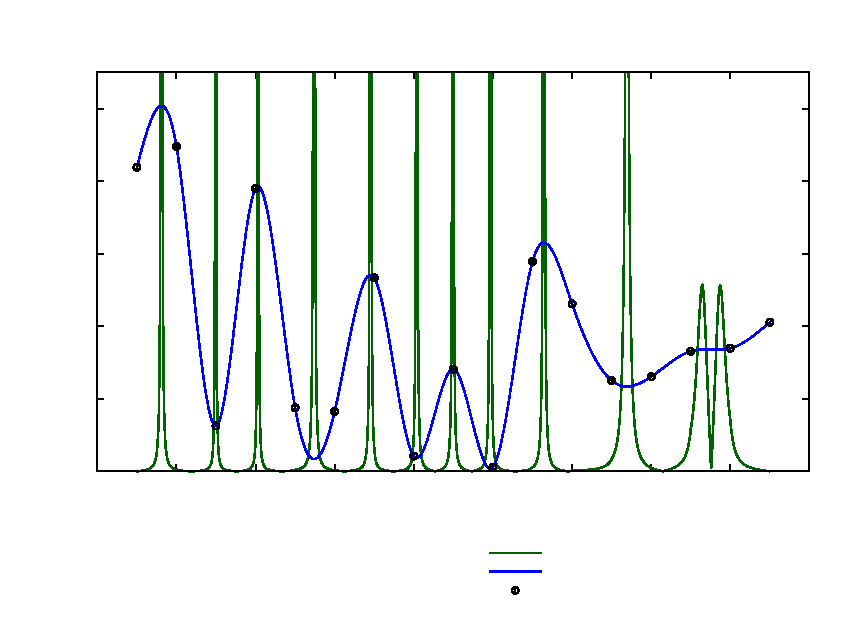
\includegraphics{./../LaTeX/graph/quest8}}%
    \gplfronttext
  \end{picture}%
\endgroup

% GNUPLOT: LaTeX picture with Postscript
\begingroup
  \fontfamily{phv}%
  \selectfont
\definecolor{t}{rgb}{0.5,0.5,0.5}
  \makeatletter
  \providecommand\color[2][]{%
    \GenericError{(gnuplot) \space\space\space\@spaces}{%
      Package color not loaded in conjunction with
      terminal option `colourtext'%
    }{See the gnuplot documentation for explanation.%
    }{Either use 'blacktext' in gnuplot or load the package
      color.sty in LaTeX.}%
    \renewcommand\color[2][]{}%
  }%
  \providecommand\includegraphics[2][]{%
    \GenericError{(gnuplot) \space\space\space\@spaces}{%
      Package graphicx or graphics not loaded%
    }{See the gnuplot documentation for explanation.%
    }{The gnuplot epslatex terminal needs graphicx.sty or graphics.sty.}%
    \renewcommand\includegraphics[2][]{}%
  }%
  \providecommand\rotatebox[2]{#2}%
  \@ifundefined{ifGPcolor}{%
    \newif\ifGPcolor
    \GPcolortrue
  }{}%
  \@ifundefined{ifGPblacktext}{%
    \newif\ifGPblacktext
    \GPblacktextfalse
  }{}%
  % define a \g@addto@macro without @ in the name:
  \let\gplgaddtomacro\g@addto@macro
  % define empty templates for all commands taking text:
  \gdef\gplbacktext{}%
  \gdef\gplfronttext{}%
  \makeatother
  \ifGPblacktext
    % no textcolor at all
    \def\colorrgb#1{}%
    \def\colorgray#1{}%
  \else
    % gray or color?
    \ifGPcolor
      \def\colorrgb#1{\color[rgb]{#1}}%
      \def\colorgray#1{\color[gray]{#1}}%
      \expandafter\def\csname LTw\endcsname{\color{white}}%
      \expandafter\def\csname LTb\endcsname{\color{black}}%
      \expandafter\def\csname LTa\endcsname{\color{black}}%
      \expandafter\def\csname LT0\endcsname{\color[rgb]{1,0,0}}%
      \expandafter\def\csname LT1\endcsname{\color[rgb]{0,1,0}}%
      \expandafter\def\csname LT2\endcsname{\color[rgb]{0,0,1}}%
      \expandafter\def\csname LT3\endcsname{\color[rgb]{1,0,1}}%
      \expandafter\def\csname LT4\endcsname{\color[rgb]{0,1,1}}%
      \expandafter\def\csname LT5\endcsname{\color[rgb]{1,1,0}}%
      \expandafter\def\csname LT6\endcsname{\color[rgb]{0,0,0}}%
      \expandafter\def\csname LT7\endcsname{\color[rgb]{1,0.3,0}}%
      \expandafter\def\csname LT8\endcsname{\color[rgb]{0.5,0.5,0.5}}%
    \else
      % gray
      \def\colorrgb#1{\color{black}}%
      \def\colorgray#1{\color[gray]{#1}}%
      \expandafter\def\csname LTw\endcsname{\color{white}}%
      \expandafter\def\csname LTb\endcsname{\color{black}}%
      \expandafter\def\csname LTa\endcsname{\color{black}}%
      \expandafter\def\csname LT0\endcsname{\color{black}}%
      \expandafter\def\csname LT1\endcsname{\color{black}}%
      \expandafter\def\csname LT2\endcsname{\color{black}}%
      \expandafter\def\csname LT3\endcsname{\color{black}}%
      \expandafter\def\csname LT4\endcsname{\color{black}}%
      \expandafter\def\csname LT5\endcsname{\color{black}}%
      \expandafter\def\csname LT6\endcsname{\color{black}}%
      \expandafter\def\csname LT7\endcsname{\color{black}}%
      \expandafter\def\csname LT8\endcsname{\color{black}}%
    \fi
  \fi
  \setlength{\unitlength}{0.0500bp}%
  \begin{picture}(7936.00,5668.00)%
    \gplgaddtomacro\gplbacktext{%
      \csname LTb\endcsname%
      \put(1002,1472){\makebox(0,0){\strut{} 0}}%
      \put(1611,1363){\makebox(0,0){\strut{} 0.2}}%
      \put(2219,1254){\makebox(0,0){\strut{} 0.4}}%
      \put(2828,1145){\makebox(0,0){\strut{} 0.6}}%
      \put(3436,1036){\makebox(0,0){\strut{} 0.8}}%
      \put(4044,926){\makebox(0,0){\strut{} 1}}%
      \put(4652,817){\makebox(0,0){\strut{} 1.2}}%
      \put(4833,867){\makebox(0,0){\strut{}-1}}%
      \put(5024,970){\makebox(0,0){\strut{} 0}}%
      \put(5216,1074){\makebox(0,0){\strut{} 1}}%
      \put(5408,1177){\makebox(0,0){\strut{} 2}}%
      \put(5599,1280){\makebox(0,0){\strut{} 3}}%
      \put(5791,1383){\makebox(0,0){\strut{} 4}}%
      \put(5982,1486){\makebox(0,0){\strut{} 5}}%
      \put(6174,1589){\makebox(0,0){\strut{} 6}}%
      \put(6366,1692){\makebox(0,0){\strut{} 7}}%
      \put(6557,1796){\makebox(0,0){\strut{} 8}}%
      \put(6749,1899){\makebox(0,0){\strut{} 9}}%
      \put(6941,2002){\makebox(0,0){\strut{} 10}}%
      \put(963,2307){\makebox(0,0)[r]{\strut{} 0}}%
      \put(963,2458){\makebox(0,0)[r]{\strut{} 1}}%
      \put(963,2609){\makebox(0,0)[r]{\strut{} 2}}%
      \put(963,2760){\makebox(0,0)[r]{\strut{} 3}}%
      \put(963,2912){\makebox(0,0)[r]{\strut{} 4}}%
      \put(963,3062){\makebox(0,0)[r]{\strut{} 5}}%
      \put(963,3213){\makebox(0,0)[r]{\strut{} 6}}%
      \put(963,3364){\makebox(0,0)[r]{\strut{} 7}}%
      \put(963,3516){\makebox(0,0)[r]{\strut{} 8}}%
      \put(963,3667){\makebox(0,0)[r]{\strut{} 9}}%
      \put(963,3818){\makebox(0,0)[r]{\strut{} 10}}%
      \put(3968,5325){\makebox(0,0){\strut{}Ajuste com Splines 3D}}%
    }%
    \gplgaddtomacro\gplfronttext{%
      \put(5009,630){\makebox(0,0)[r]{\strut{}splines3D}}%
      \csname LTb\endcsname%
      \put(5009,450){\makebox(0,0)[r]{\strut{}data points}}%
      \csname LTb\endcsname%
      \put(2388,939){\makebox(0,0){\strut{}t}}%
      \put(6706,1299){\makebox(0,0){\strut{}y(t)}}%
    }%
    \gplbacktext
    \put(0,0){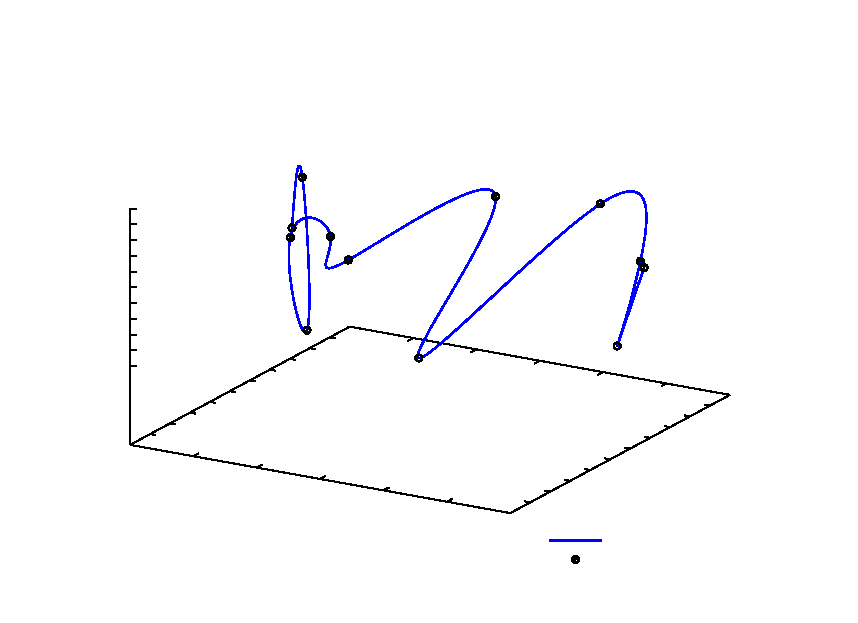
\includegraphics{./../LaTeX/graph/quest9}}%
    \gplfronttext
  \end{picture}%
\endgroup

\section{Códigos}

\paragraph{}Os códigos desenvolvidos estão em anexo. Todos os algoritmos foram
implementados em C usando-se apenas as bibliotecas padrões da linguagem. 
Cada questão que exigiu um código tem uma arquivo fonte chamado questX.c que pode
ser compilado com "gcc -Wall questX.c -o questX -lm". Existem algumas funções comuns
a todos esses arquivos que estão definidas em bibliotecas, são elas:
\begin{itemize}
  \item matrix-class.h : define a estrutura de matriz e operações
  básicas como criação, deleção, adição e transposição.
  \item usual-math.h : define algumas funções básicas como módulo, máx
  \item LU-fatoration.h: implementa a fatoração LU com permutação. Amplamente
  utilizada para inverter matrizes e resolver sistemas
  \item simply-gaussian-elimination.h : implementa eliminação gaussiana com permutação.
  \item inversa.h : calcula a matriz inversa como sugerido na lista 3.
  \item determinante.h: calcula o determinante como sugerido na lista 3  
  \item Jacobi-method.h: soluciona sistema por método iterativo de Jacobi
  \item Gauss-Seidel-method.h : soluciona sistema por método iterativo de Gauss-Seidel
  \item AlgebricSystem.h: implementa método vetorial de Newton para 2 dimensões
  \item DataFitting.h : funções de interpolação polinomial 
\end{itemize}

\paragraph{}Essas bibliotecas são comuns a todas as questões e foram desenvolvidas
ao longo do curso. Como algumas questões usam ideias parecidas pode haver repetição
de algumas rotinas em alguns .c. Isso ocorre pois cada .c é independente e pode
ser compilado separadamente.


\end{document}
